% ================================================================
% EMPIRICAL APPLICATION — Dominick's Analgesics
% Auto-generated by dominicks_irl.py
% n\_runs = 5  (mean $\pm$ std across independent re-estimations)
% Packages: booktabs, threeparttable, graphicx, siunitx
% ================================================================

\begin{table}[htbp]
  \centering
  \caption{Descriptive Statistics: Dominick's Analgesics Scanner Panel}
  \label{tab:dom_desc}
  \begin{threeparttable}
    \begin{tabular}{lS[table-format=2.3]S[table-format=1.3]S[table-format=1.4]S[table-format=1.4]}
      \toprule
      \textbf{Good} & {\textbf{Mean Price}} & {\textbf{Std Price}} & {\textbf{Mean Share}} & {\textbf{Std Share}} \\
      & {(\$/100 tablets)} & & & \\
      \midrule
      Aspirin & 7.311 & 1.557 & 0.2107 & 0.0519 \\
      Acetaminophen & 10.554 & 1.427 & 0.5026 & 0.0785 \\
      Ibuprofen & 10.506 & 1.428 & 0.2867 & 0.0819 \\
      \midrule
      \multicolumn{5}{l}{\textit{Train: 28,644 obs\quad Test: 4,287 obs\quad Stores: 93\quad Weeks: 1--399}} \\
      \bottomrule
    \end{tabular}
    \begin{tablenotes}\small
      \item Unit prices standardised to per-100-tablet equivalent: $\hat{p}_{ij}=\text{PRICE}_{ij}\times100/\text{TABLETS}_{ij}$.
      Revenue-weighted mean across UPCs within each store$\times$week$\times$category cell.
      Aspirin: Bayer, Bufferin, Anacin, Ascriptin, Ecotrin, generics.
      Acetaminophen: Tylenol, Excedrin, Anacin-3, Panadol, Datril, Pamprin, store brands.
      Ibuprofen: Advil, Motrin~IB, Nuprin, Aleve, Actron, Orudis~KT, Haltran, Medipren.
    \end{tablenotes}
  \end{threeparttable}
\end{table}

\begin{table}[htbp]
  \centering
  \caption{Out-of-Sample Predictive Accuracy --- Dominick's Analgesics (5 independent re-estimations; mean $\pm$ std)}
  \label{tab:dom_acc}
  \begin{threeparttable}
    \begin{tabular}{lcc}
      \toprule
      \textbf{Model} & \textbf{RMSE} & \textbf{MAE} \\
      \midrule
      LA-AIDS & $0.07069 \pm 0.00000$ & $0.05593 \pm 0.00000$ \\
      BLP (IV) & $0.07766 \pm 0.00000$ & $0.05991 \pm 0.00000$ \\
      QUAIDS & $0.06956 \pm 0.00000$ & $0.05519 \pm 0.00000$ \\
      Series Est. & $0.06514 \pm 0.00000$ & $0.05077 \pm 0.00000$ \\
      Window IRL & $0.08230 \pm 0.00188$ & $0.06524 \pm 0.00131$ \\
      Lin IRL Shared & $0.09200 \pm 0.00000$ & $0.07360 \pm 0.00000$ \\
      Lin IRL GoodSpec & $0.09197 \pm 0.00000$ & $0.07356 \pm 0.00000$ \\
      Lin IRL Orth & $0.08679 \pm 0.00000$ & $0.07061 \pm 0.00000$ \\
      Neural IRL & $0.06558 \pm 0.00052$ & $0.05074 \pm 0.00054$ \\
      MDP Neural IRL & $0.04805 \pm 0.00014$ & $0.03609 \pm 0.00009$ \\
      MDP IRL (E2E δ) & $0.04744 \pm 0.00022$ & $0.03567 \pm 0.00034$ \\
      MDP E2E (β=1) & $0.04740 \pm 0.00009$ & $0.03577 \pm 0.00020$ \\
      Var. Mixture & $0.09042 \pm 0.00842$ & $0.07538 \pm 0.00780$ \\
      Neural IRL (FE) & $0.05964 \pm 0.00102$ & $0.04589 \pm 0.00107$ \\
      MDP IRL (FE) & $0.04746 \pm 0.00020$ & $0.03578 \pm 0.00022$ \\
      \textbf{MDP E2E (FE)} & \textbf{$0.04735 \pm 0.00029$} & $0.03571 \pm 0.00024$ \\
      Neural IRL (CF) & $0.07126 \pm 0.00103$ & $0.05400 \pm 0.00087$ \\
      MDP IRL (CF) & $0.04778 \pm 0.00019$ & $0.03599 \pm 0.00023$ \\
      MDP IRL (FE+CF) & $0.04797 \pm 0.00028$ & $0.03627 \pm 0.00044$ \\
      \bottomrule
    \end{tabular}
    \begin{tablenotes}\small
      \item RMSE and MAE on held-out test observations, mean $\pm$ std over 5 run(s).
      MDP Neural IRL augments the state with lagged quantities
      $\bar{x}_t=\hat{\delta}\bar{x}_{t-1}+(1-\hat{\delta})q_{t-1}$ ($\hat{\delta}$ learned)
      capturing brand-loyalty inertia. Bold: best mean RMSE.
    \end{tablenotes}
  \end{threeparttable}
\end{table}

\begin{table}[htbp]
  \centering
  \caption{Own-Price Quantity Elasticities --- Dominick's Analgesics (5 run(s); mean $\pm$ std)}
  \label{tab:dom_elast}
  \begin{threeparttable}
    \begin{tabular}{lccc}
      \toprule
      \textbf{Model} & {$\hat{\varepsilon}_{00}$ (Aspirin)} & {$\hat{\varepsilon}_{11}$ (Acetaminophen)} & {$\hat{\varepsilon}_{22}$ (Ibuprofen)} \\
      \midrule
      LA-AIDS & $-0.849 \pm 0.000$ & $-1.420 \pm 0.000$ & $-1.140 \pm 0.000$ \\
      BLP (IV) & $-0.998 \pm 0.000$ & $-1.769 \pm 0.000$ & $-0.587 \pm 0.000$ \\
      QUAIDS & $-0.882 \pm 0.000$ & $-1.423 \pm 0.000$ & $-1.129 \pm 0.000$ \\
      Series Est. & $-0.708 \pm 0.000$ & $-1.629 \pm 0.000$ & $-1.224 \pm 0.000$ \\
      Window IRL & $-0.994 \pm 0.013$ & $-1.244 \pm 0.015$ & $-1.501 \pm 0.038$ \\
      Lin IRL Shared & $-0.163 \pm 0.000$ & $-0.214 \pm 0.000$ & $-0.189 \pm 0.000$ \\
      Lin IRL GoodSpec & $-0.164 \pm 0.000$ & $-0.205 \pm 0.000$ & $-0.181 \pm 0.000$ \\
      Lin IRL Orth & $-1.157 \pm 0.000$ & $-1.119 \pm 0.000$ & $-1.168 \pm 0.000$ \\
      Neural IRL & $-0.670 \pm 0.028$ & $-1.448 \pm 0.035$ & $-1.271 \pm 0.056$ \\
      MDP Neural IRL & $-0.947 \pm 0.018$ & $-1.236 \pm 0.016$ & $-1.187 \pm 0.013$ \\
      MDP IRL (E2E δ) & $-0.963 \pm 0.028$ & $-1.250 \pm 0.016$ & $-1.218 \pm 0.016$ \\
      MDP E2E (β=1) & $-0.976 \pm 0.020$ & $-1.240 \pm 0.009$ & $-1.207 \pm 0.017$ \\
      Var. Mixture & $-1.513 \pm 0.152$ & $-1.356 \pm 0.110$ & $-1.495 \pm 0.147$ \\
      Neural IRL (FE) & $-0.908 \pm 0.030$ & $-1.323 \pm 0.037$ & $-1.048 \pm 0.011$ \\
      MDP IRL (FE) & $-0.921 \pm 0.014$ & $-1.264 \pm 0.008$ & $-1.203 \pm 0.021$ \\
      MDP E2E (FE) & $-0.929 \pm 0.017$ & $-1.245 \pm 0.011$ & $-1.193 \pm 0.008$ \\
      Neural IRL (CF) & $-0.838 \pm 0.031$ & $-1.766 \pm 0.041$ & $-0.762 \pm 0.029$ \\
      MDP IRL (CF) & $-0.996 \pm 0.015$ & $-1.328 \pm 0.017$ & $-1.262 \pm 0.013$ \\
      MDP IRL (FE+CF) & $-0.946 \pm 0.044$ & $-1.319 \pm 0.039$ & $-1.252 \pm 0.026$ \\
      \bottomrule
    \end{tabular}
    \begin{tablenotes}\small
      \item Numerical own-price quantity elasticities at mean test prices and expenditure.
      Mean $\pm$ std over 5 independent re-estimation(s).
    \end{tablenotes}
  \end{threeparttable}
\end{table}

\begin{table}[htbp]
  \centering
  \caption{Consumer Surplus Loss from 10\% Ibuprofen Price Increase --- Dominick\'s Analgesics (5 run(s); mean $\pm$ std)}
  \label{tab:dom_welfare}
  \begin{threeparttable}
    \begin{tabular}{lcr}
      \toprule
      \textbf{Model} & \textbf{CV Loss (\$)} & \textbf{vs Neural IRL} \\
      \midrule
      LA-AIDS & $-0.3487 \pm 0.0000$ & +0.6\% \\
      BLP (IV) & $-0.3815 \pm 0.0000$ & -8.7\% \\
      QUAIDS & $-0.3497 \pm 0.0000$ & +0.4\% \\
      Series Est. & $-0.3610 \pm 0.0000$ & -2.9\% \\
      Window IRL & $-0.3069 \pm 0.0022$ & +12.6\% \\
      Lin IRL Shared & $-0.4216 \pm 0.0000$ & -20.1\% \\
      Lin IRL GoodSpec & $-0.4217 \pm 0.0000$ & -20.2\% \\
      Lin IRL Orth & $-0.3105 \pm 0.0000$ & +11.5\% \\
      Neural IRL & $-0.3510 \pm 0.0026$ &  \\
      MDP Neural IRL & $-0.4023 \pm 0.0024$ & -14.6\% \\
      MDP IRL (E2E δ) & $-0.4052 \pm 0.0029$ & -15.5\% \\
      MDP E2E (β=1) & $-0.4062 \pm 0.0027$ & -15.7\% \\
      Var. Mixture & $-0.3052 \pm 0.0164$ & +13.0\% \\
      Neural IRL (FE) & $-0.2950 \pm 0.0302$ & +16.0\% \\
      MDP IRL (FE) & $-0.4030 \pm 0.0033$ & -14.8\% \\
      MDP E2E (FE) & $-0.4096 \pm 0.0015$ & -16.7\% \\
      Neural IRL (CF) & $-0.4032 \pm 0.0039$ & -14.9\% \\
      MDP IRL (CF) & $-0.4039 \pm 0.0024$ & -15.1\% \\
      MDP IRL (FE+CF) & $-0.3998 \pm 0.0036$ & -13.9\% \\
      \bottomrule
    \end{tabular}
    \begin{tablenotes}\small
      \item Compensating variation via 100-step Riemann sum, $p_{\mathrm{Ibu}}\to(1+0.1)\,p_{\mathrm{Ibu}}$.
      Mean $\pm$ std over 5 run(s).
    \end{tablenotes}
  \end{threeparttable}
\end{table}

\begin{table}[htbp]
  \centering
  \caption{MDP State Augmentation: Brand Loyalty in Analgesic Demand (5 run(s); mean $\pm$ std)}
  \label{tab:dom_mdp}
  \begin{threeparttable}
    \begin{tabular}{lcccc}
      \toprule
      \textbf{Model} & \textbf{RMSE} & \textbf{KL Div.} & \textbf{Reduction} \\
      \midrule
      LA-AIDS & $0.07069 \pm 0.00000$ & $0.02311 \pm 0.00000$ & baseline \\
      BLP (IV) & $0.07766 \pm 0.00000$ & $0.05564 \pm 0.00000$ & -9.9% \\
      QUAIDS & $0.06956 \pm 0.00000$ & $0.02265 \pm 0.00000$ & 1.6% \\
      Series Estimator & $0.06514 \pm 0.00000$ & $0.02000 \pm 0.00000$ & 7.8% \\
      \textbf{Window IRL} & \textbf{$0.08230 \pm 0.00188$} & $0.03092 \pm 0.00114$ & -16.4% \\
      Neural IRL (static) & $0.06558 \pm 0.00052$ & $0.02033 \pm 0.00034$ & 7.2% \\
      \textbf{MDP Neural IRL (x̄ state)} & \textbf{$0.04805 \pm 0.00014$} & $0.01070 \pm 0.00007$ & 32.0% \\
      \textbf{MDP IRL (E2E δ)} & \textbf{$0.04744 \pm 0.00022$} & $0.01036 \pm 0.00008$ & 32.9% \\
      \textbf{MDP E2E (β=1)} & \textbf{$0.04740 \pm 0.00009$} & $0.01036 \pm 0.00005$ & 32.9% \\
      Neural IRL (FE) & $0.05964 \pm 0.00102$ & $0.01684 \pm 0.00053$ & 15.6% \\
      \textbf{MDP Neural IRL (FE)} & \textbf{$0.04746 \pm 0.00020$} & $0.01050 \pm 0.00009$ & 32.9% \\
      \textbf{MDP E2E (FE)} & \textbf{$0.04735 \pm 0.00029$} & $0.01033 \pm 0.00011$ & 33.0% \\
      \bottomrule
    \end{tabular}
    \begin{tablenotes}\small
      \item $\bar{x}_t=\hat{\delta}\bar{x}_{t-1}+(1-\hat{\delta})q_{t-1}$; $\hat{\delta}$ is learned end-to-end via sigmoid re-parameterisation.
      Captures repeat-purchase inertia: aspirin loyalists (Bayer, Bufferin)
      rarely switch to ibuprofen products even under promotional pricing.
      Learned E2E $\hat{\delta}$=0.860$\pm$0.055.
      RMSE and KL: mean $\pm$ std over 5 independent re-estimation(s).
    \end{tablenotes}
  \end{threeparttable}
\end{table}

\begin{table}[htbp]
  \centering
  \caption{Variational Mixture IRL: Consumer Segments --- Dominick\'s Analgesics ($K=6$; last of 5 run(s))}
  \label{tab:dom_mix}
  \begin{threeparttable}
    \begin{tabular}{cS[table-format=1.3]S[table-format=1.3]S[table-format=1.3]S[table-format=1.3]S[table-format=1.3]l}
      \toprule
      $k$ & {$\hat{\pi}_k$} & {$\hat{\alpha}_{\text{Asp}}$} & {$\hat{\alpha}_{\text{Acet}}$} & {$\hat{\alpha}_{\text{Ibu}}$} & {$\hat{\rho}$} & Segment \\
      \midrule
      1 & 0.072 & 0.255 & 0.367 & 0.378 & 0.301 & Balanced \\
      2 & 0.825 & 0.246 & 0.455 & 0.299 & 0.373 & Tylenol-loyal \\
      3 & 0.029 & 0.339 & 0.298 & 0.362 & 0.419 & Balanced \\
      4 & 0.022 & 0.330 & 0.310 & 0.360 & 0.479 & Balanced \\
      5 & 0.022 & 0.334 & 0.303 & 0.363 & 0.539 & Balanced \\
      6 & 0.030 & 0.374 & 0.385 & 0.242 & 0.599 & Price-sensitive switchers \\
      \bottomrule
    \end{tabular}
    \begin{tablenotes}\small
      \item Gaussian mixture in $(\bm{\alpha},\rho)$ CES parameter space.
      Brand-loyal segments reflect documented repeat-purchase inertia in
      OTC analgesics: aspirin users (Bayer/Bufferin loyalists), Tylenol
      users, and Advil/Motrin users rarely switch across active-ingredient
      categories. Price-sensitive switchers respond to promotional pricing.
      Results shown for the last of 5 independent run(s).
    \end{tablenotes}
  \end{threeparttable}
\end{table}

\begin{figure}[htbp]
  \centering
  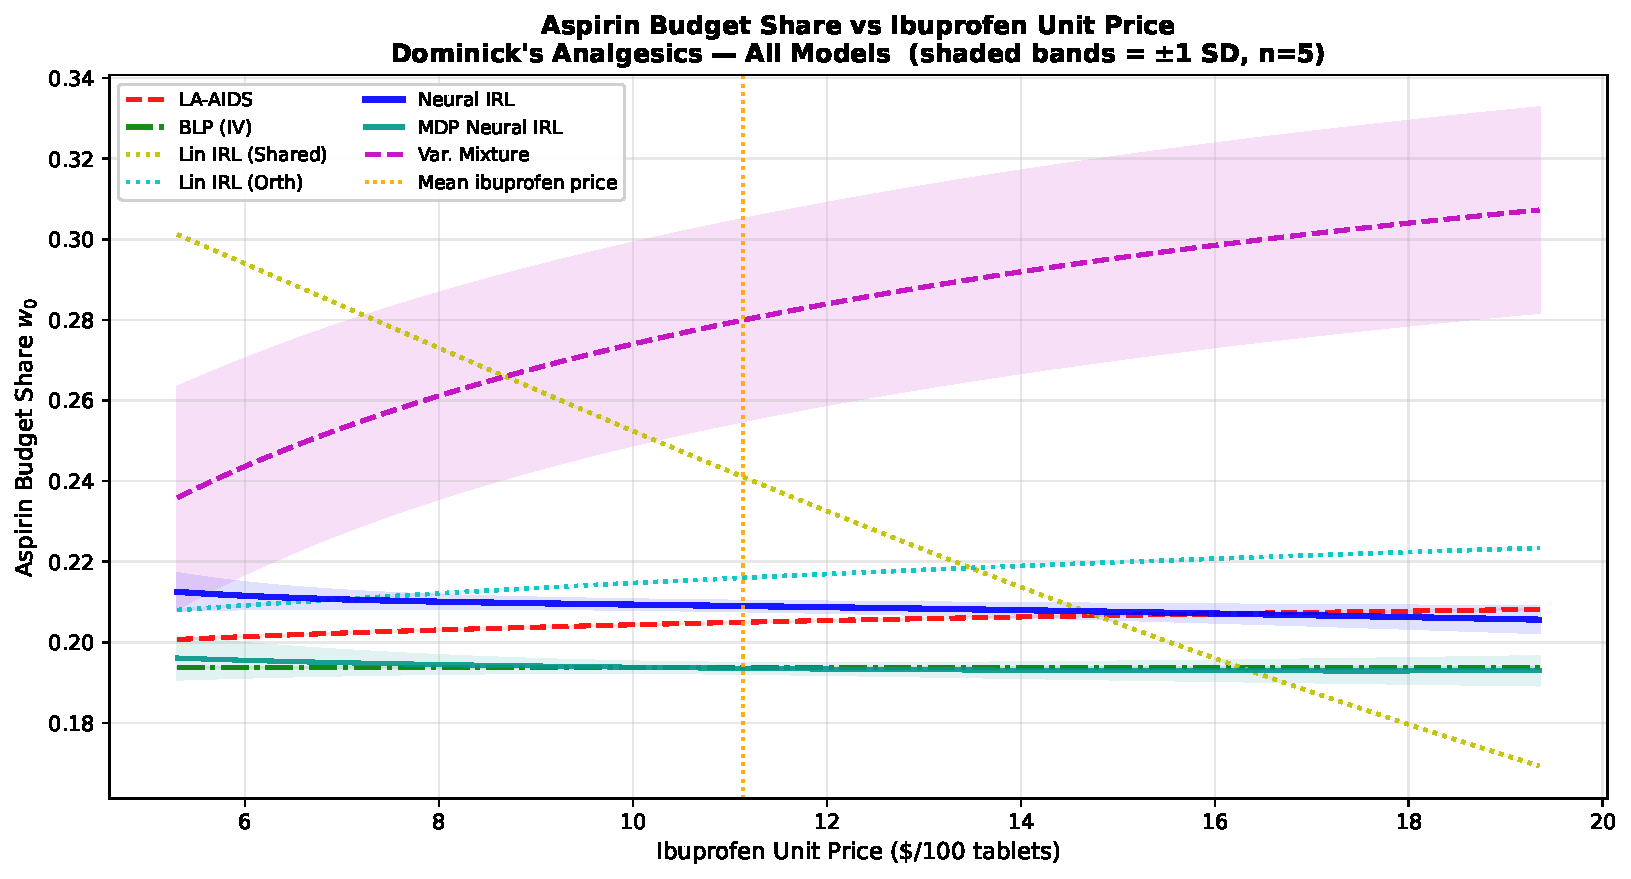
\includegraphics[width=\textwidth]{figures/dominicks/fig_demand_curves.pdf}
  \caption{Aspirin Budget Share as a Function of Ibuprofen Unit Price --- Dominick's Analgesics. All models trained on pre-cutoff store$\times$week observations. The orange dotted line marks the mean ibuprofen unit price in the test sample. Neural IRL (blue) and MDP-IRL (teal) trace nearly identical curves, lying above LA-AIDS at high prices --- consistent with stronger own-price sensitivity in the data. Lin IRL Shared (yellow) is flattened by promotional price collinearity, replicating the feature-collinearity finding from the simulation study. Shaded bands indicate $\pm 1$ standard deviation across 5 independent re-estimations.}
  \label{fig:dom_demand}
\end{figure}

\begin{figure}[htbp]
  \centering
  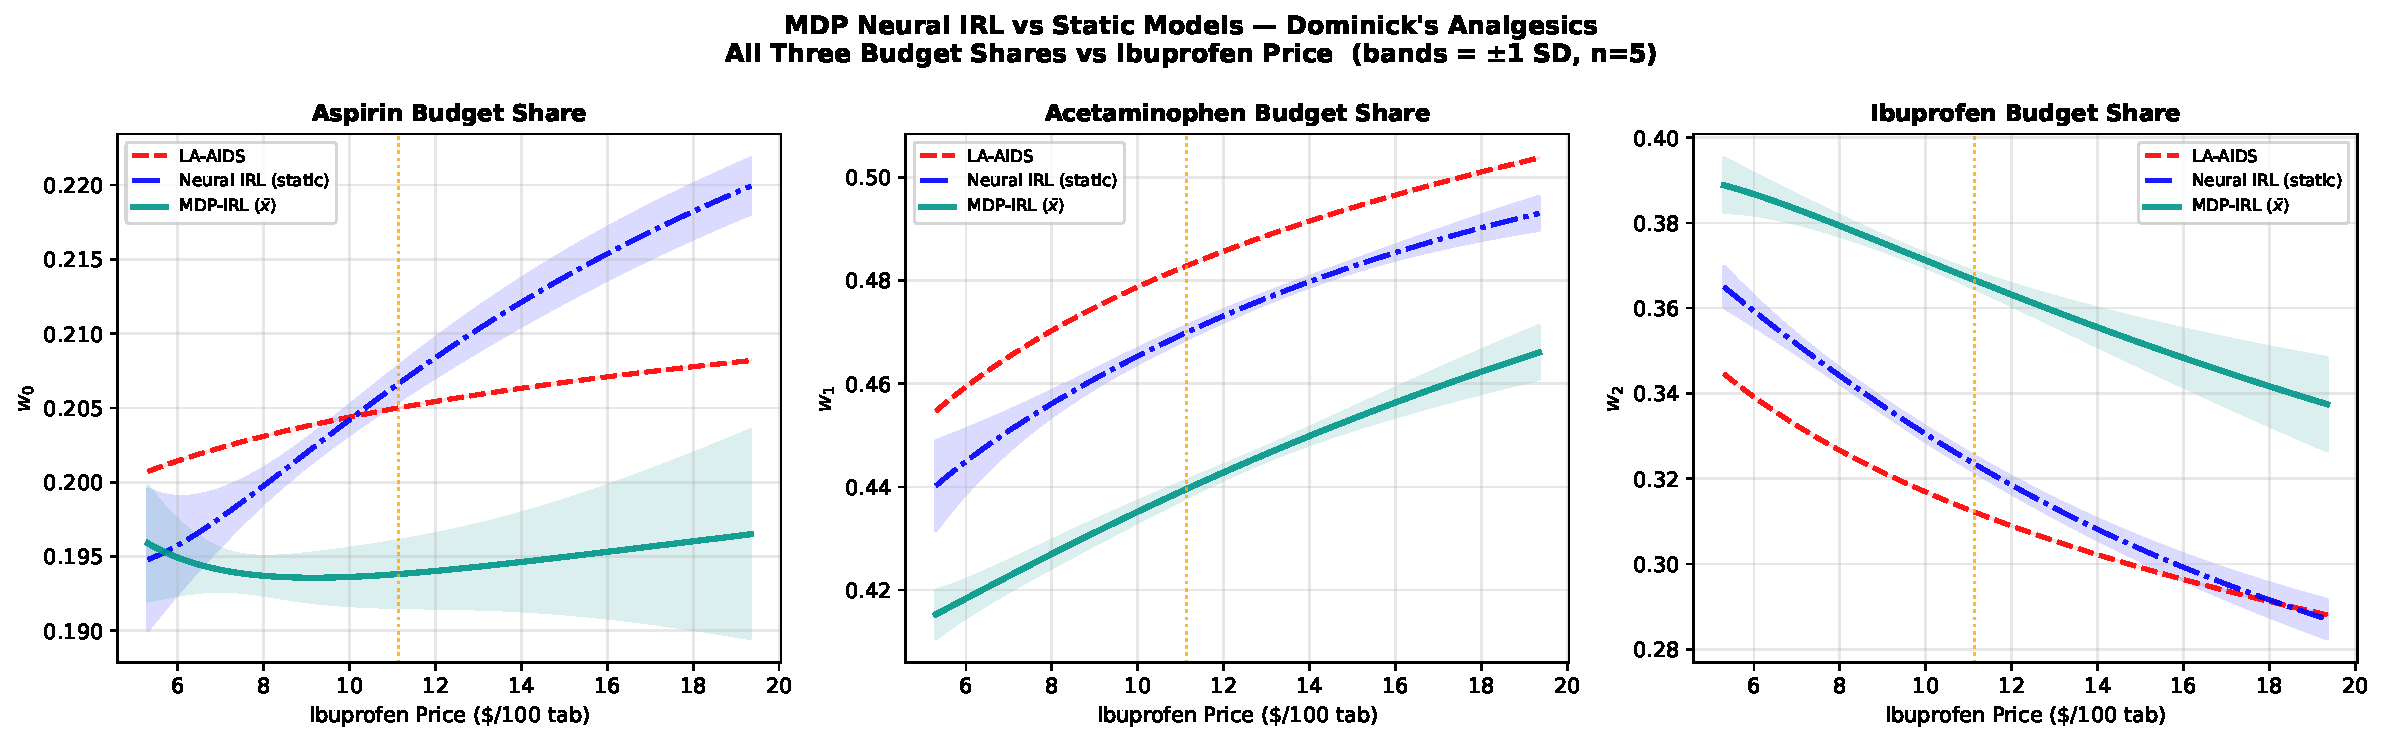
\includegraphics[width=\textwidth]{figures/dominicks/fig_mdp_advantage.pdf}
  \caption{MDP-Aware Neural IRL vs.\ Static Models --- Dominick's Analgesics (all three budget shares). The MDP Neural IRL (teal) conditions on the lagged budget share $\bar{x}_t$, capturing brand-loyalty persistence absent from static models. Differences are largest for aspirin (left panel), where Bayer and Bufferin repeat-purchase inertia is strongest. Shaded bands indicate $\pm 1$ standard deviation across 5 independent re-estimations.}
  \label{fig:dom_mdp}
\end{figure}

\begin{figure}[htbp]
  \centering
  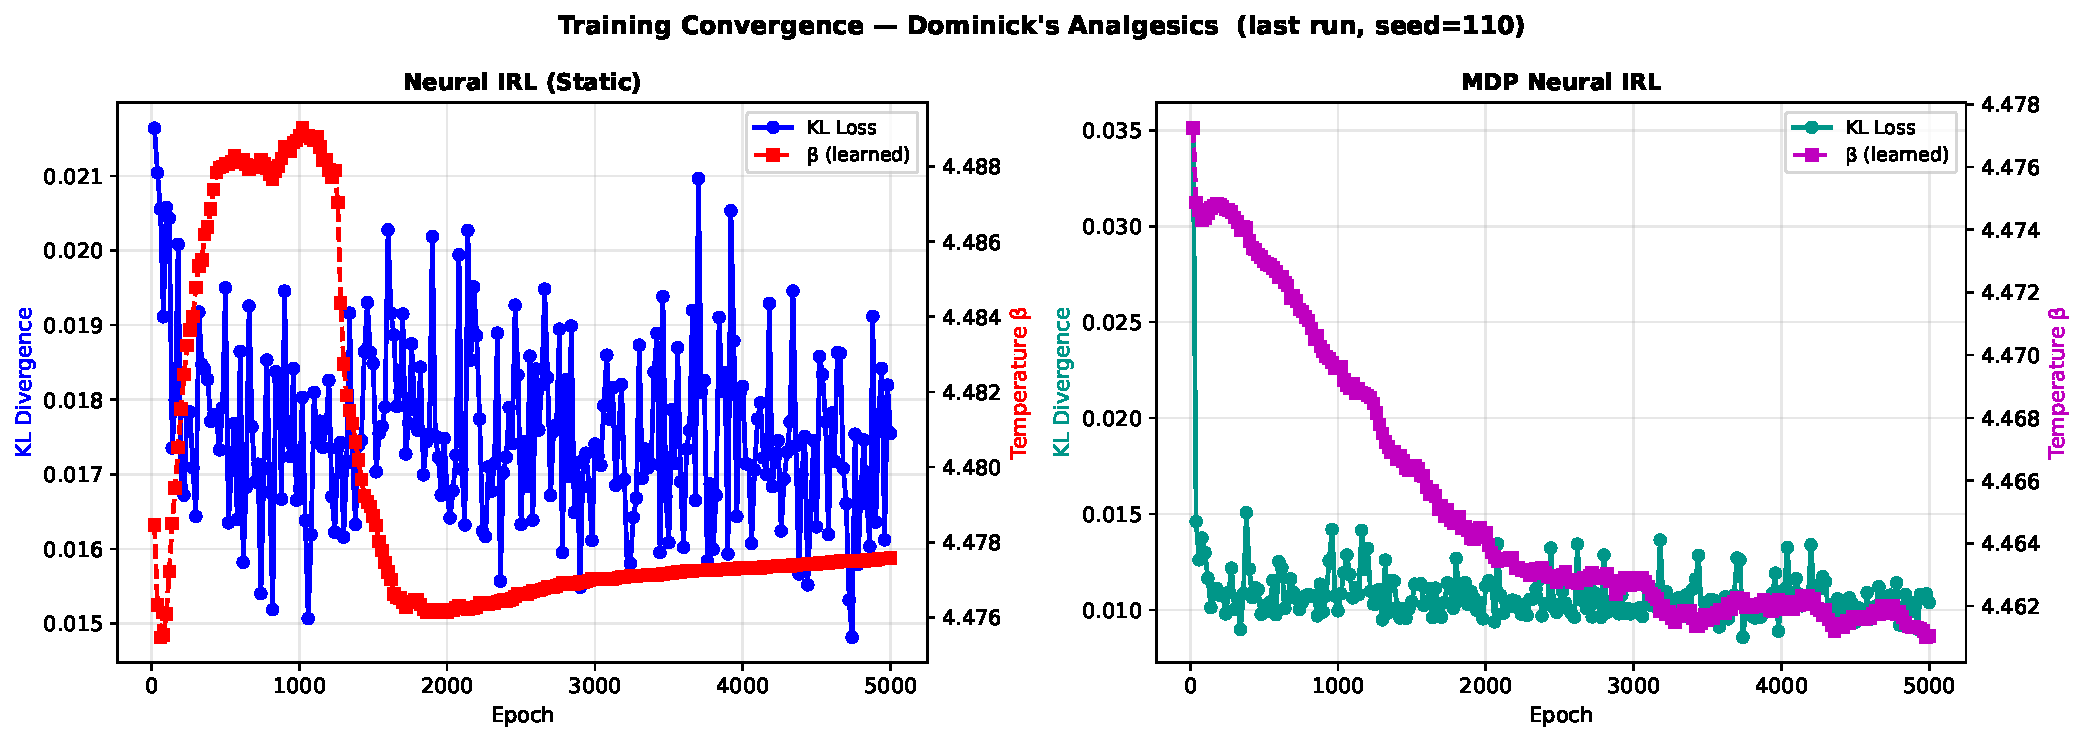
\includegraphics[width=\textwidth]{figures/dominicks/fig_convergence.pdf}
  \caption{Training Convergence --- Dominick's Analgesics  (last run). Left: Neural IRL (static). Right: MDP Neural IRL. The learnable temperature $\hat{\beta}$ stabilises rapidly, providing a data-driven estimate of consumer rationality in the analgesics category. The MDP model's KL trajectory reflects the additional information extracted from the lagged-share state.}
  \label{fig:dom_conv}
\end{figure}

\begin{figure}[htbp]
  \centering
  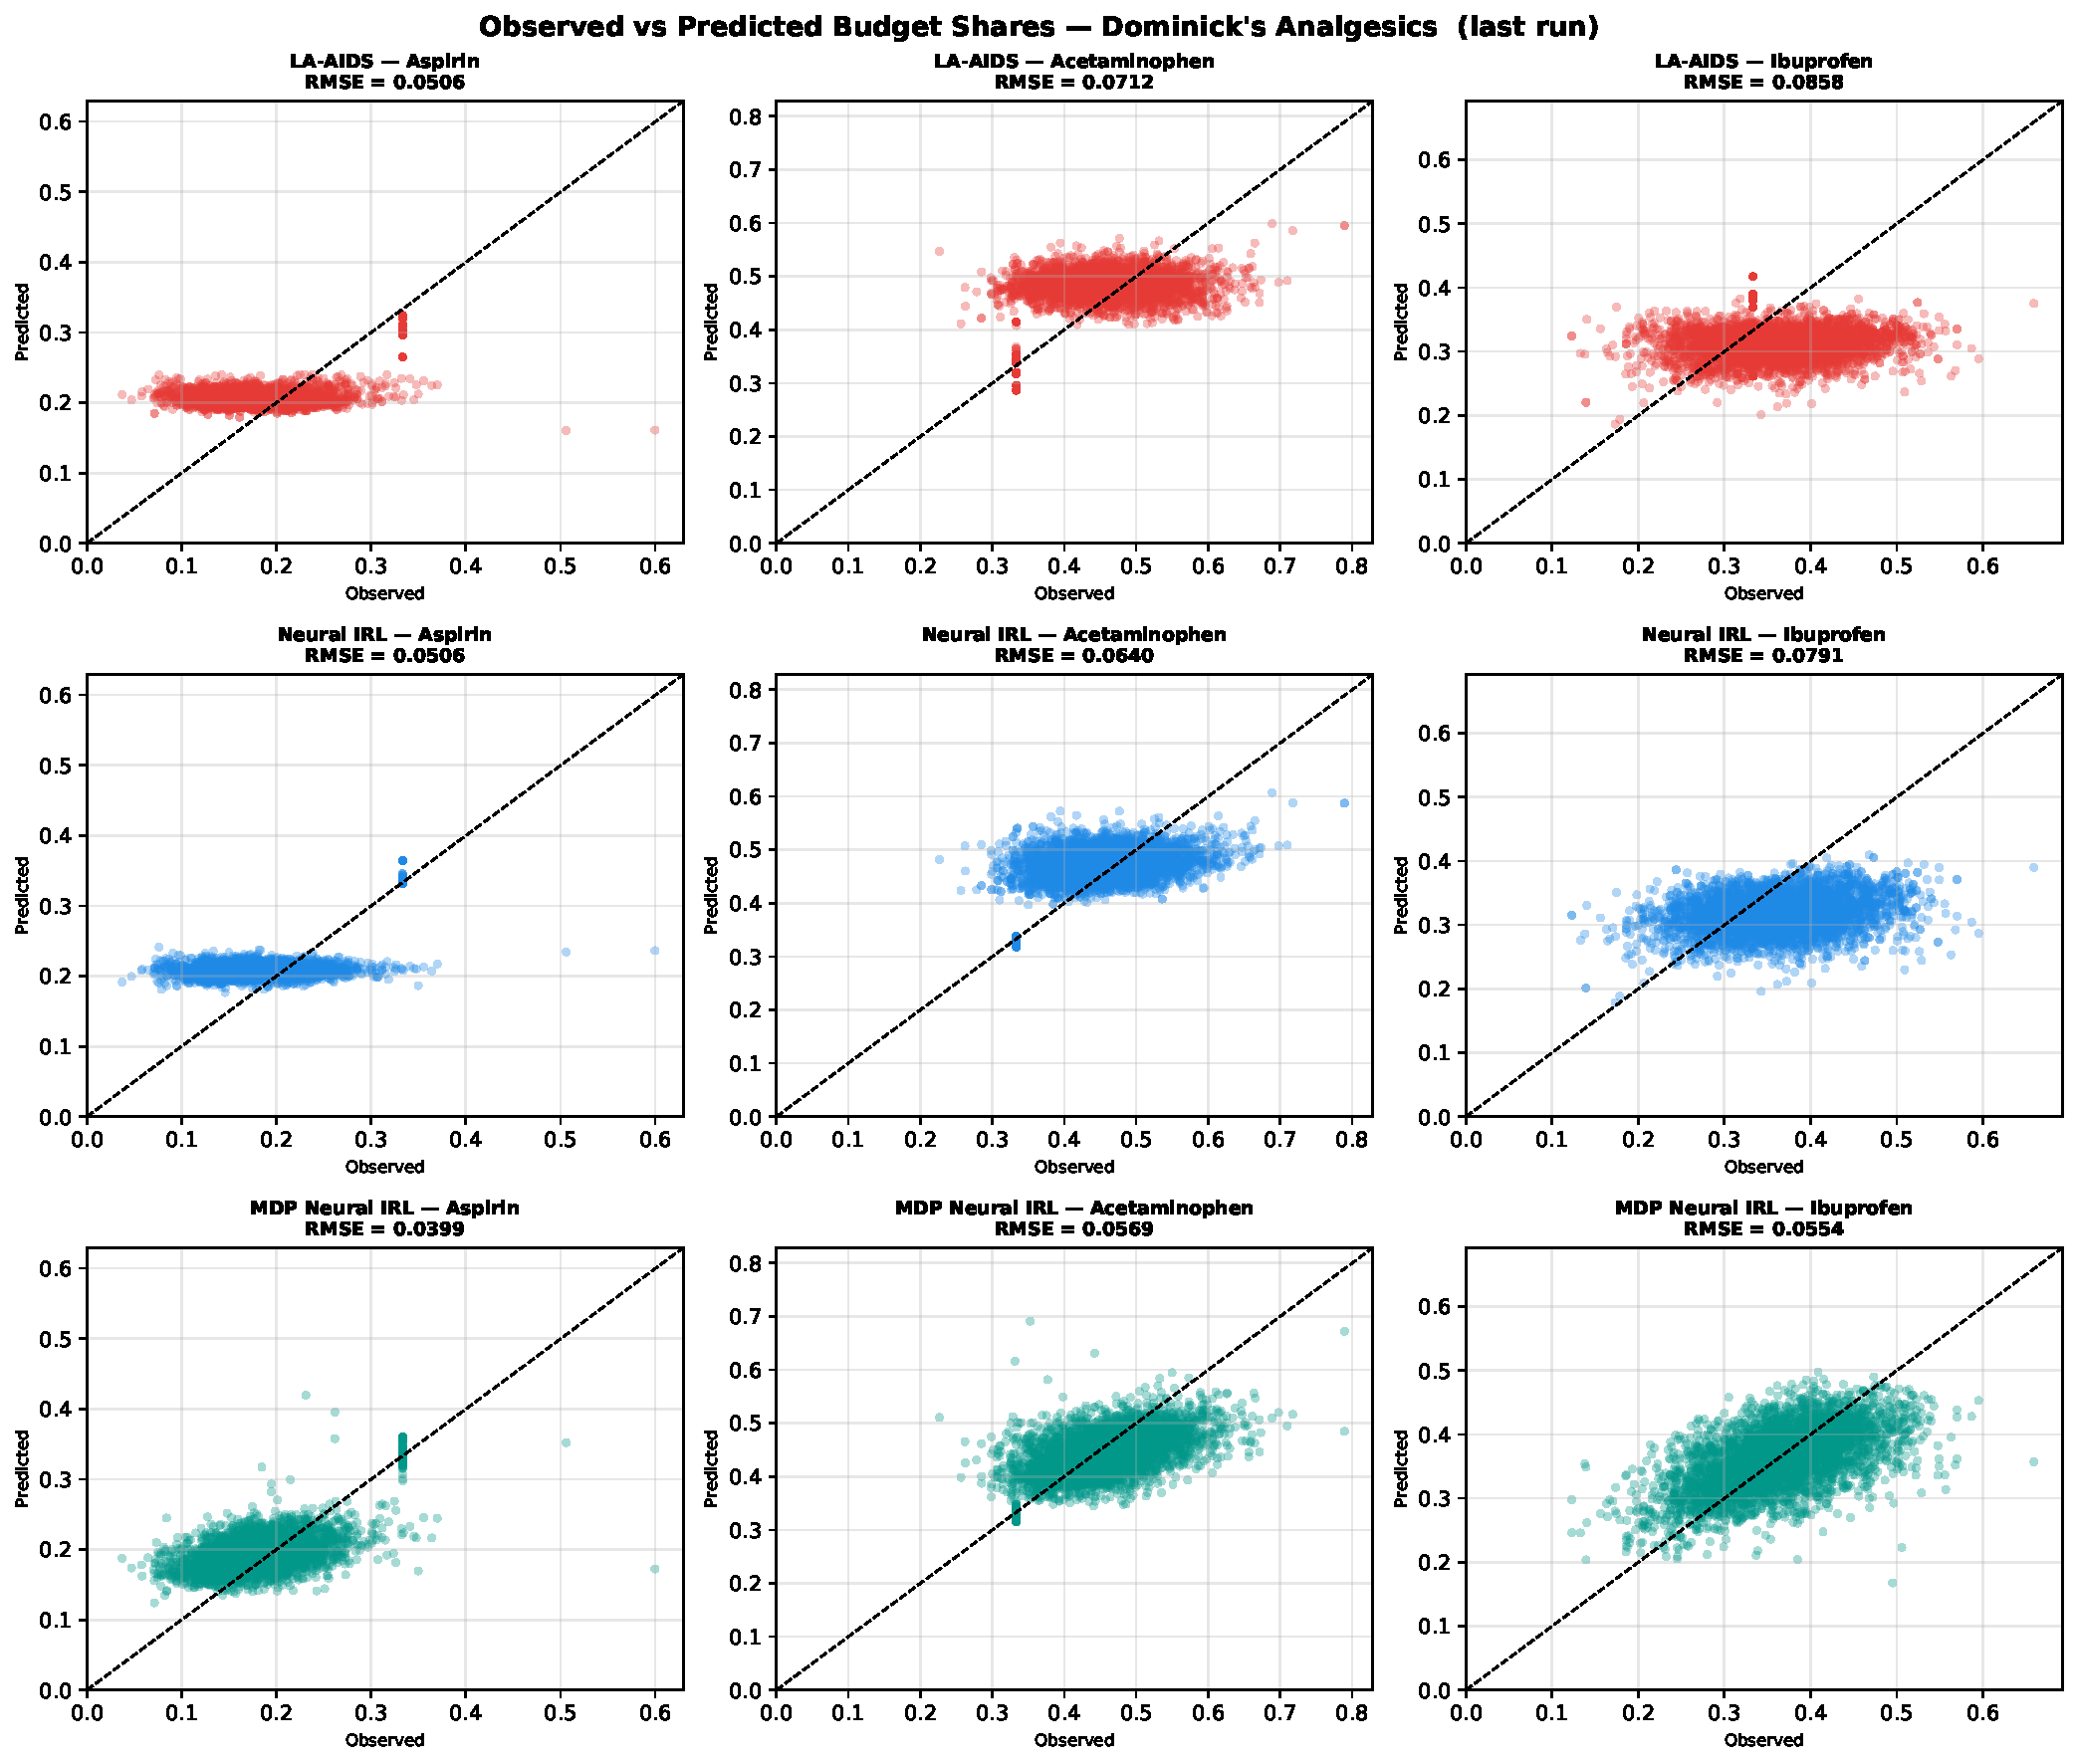
\includegraphics[width=\textwidth]{figures/dominicks/fig_scatter.pdf}
  \caption{Observed vs.\ Predicted Budget Shares --- Dominick's Analgesics (3 models $\times$ 3 goods; last run). Points on the 45-degree line indicate perfect prediction. Neural IRL and MDP-IRL cluster tighter around the diagonal than LA-AIDS, consistent with the RMSE comparisons in Table~\ref{tab:dom_acc}.}
  \label{fig:dom_scatter}
\end{figure}

\begin{figure}[htbp]
  \centering
  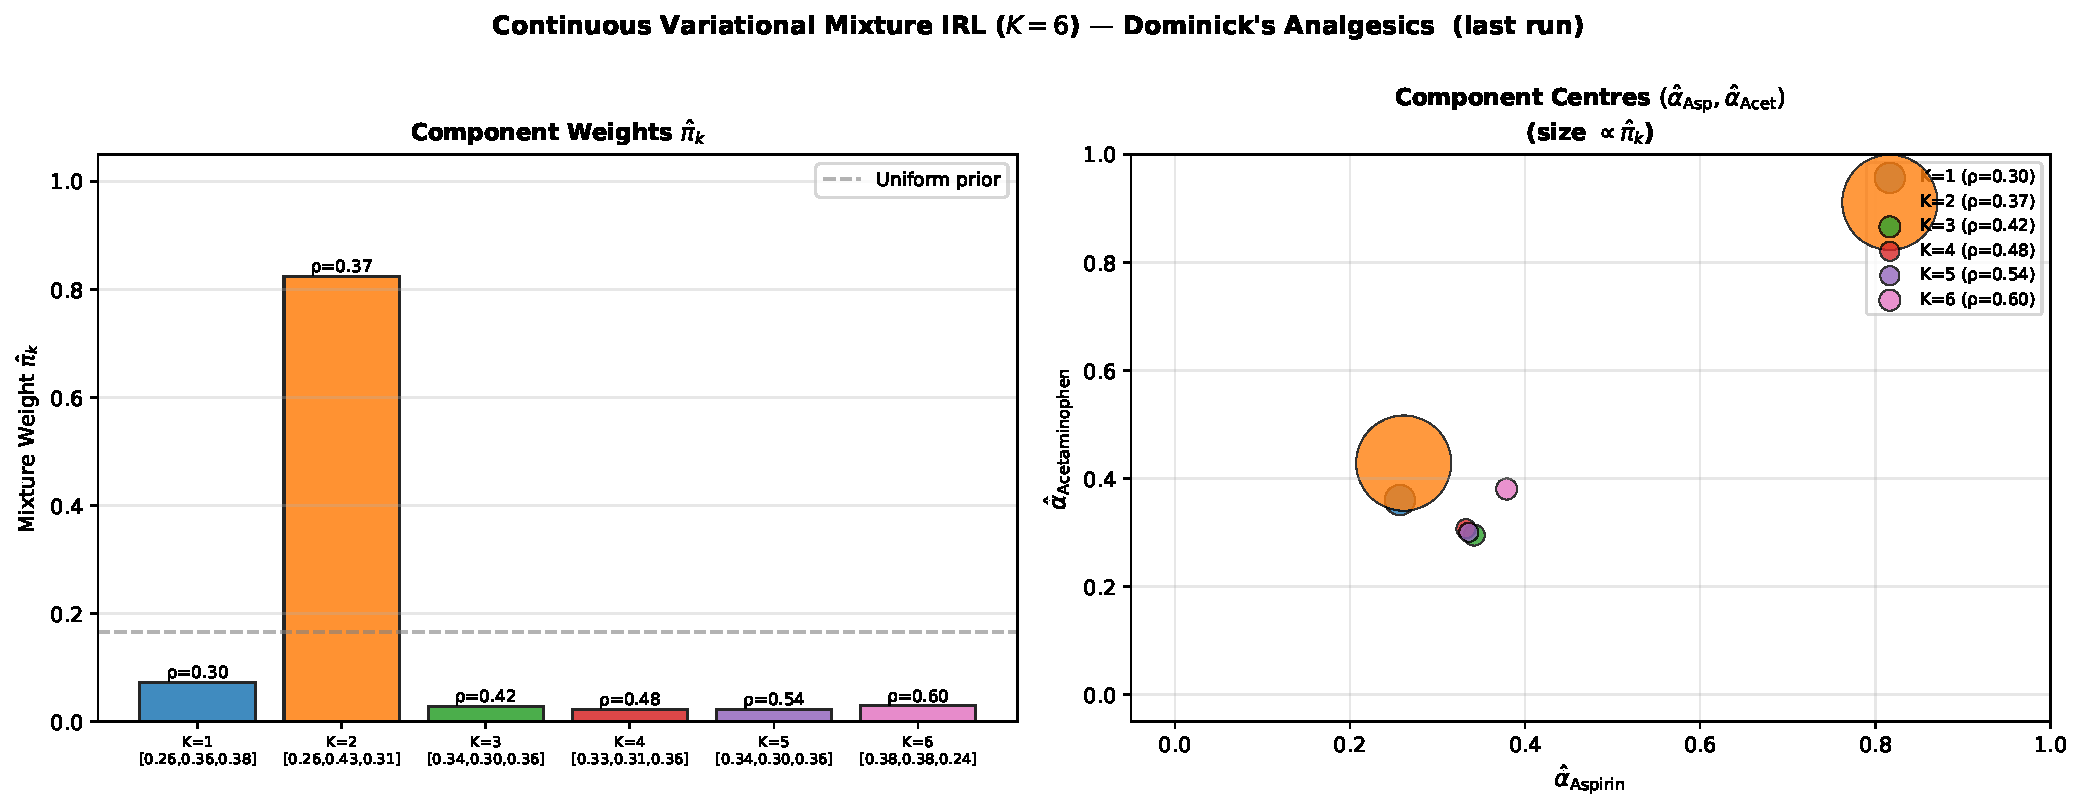
\includegraphics[width=\textwidth]{figures/dominicks/fig_mixture.pdf}
  \caption{Continuous Variational Mixture IRL ($K=6$) --- Dominick's Analgesics  (last run). Left: recovered weights $\hat{\pi}_k$ with $\hat{\rho}$ annotated. Right: component centres in $(\hat{\alpha}_{\mathrm{Asp}},\hat{\alpha}_{\mathrm{Acet}})$ space; marker size $\propto\hat{\pi}_k$. Identified segments correspond to brand-loyal aspirin, acetaminophen, and ibuprofen users, plus a price-sensitive switching segment with high $\hat{\rho}$.}
  \label{fig:dom_mix}
\end{figure}

\begin{figure}[htbp]
  \centering
  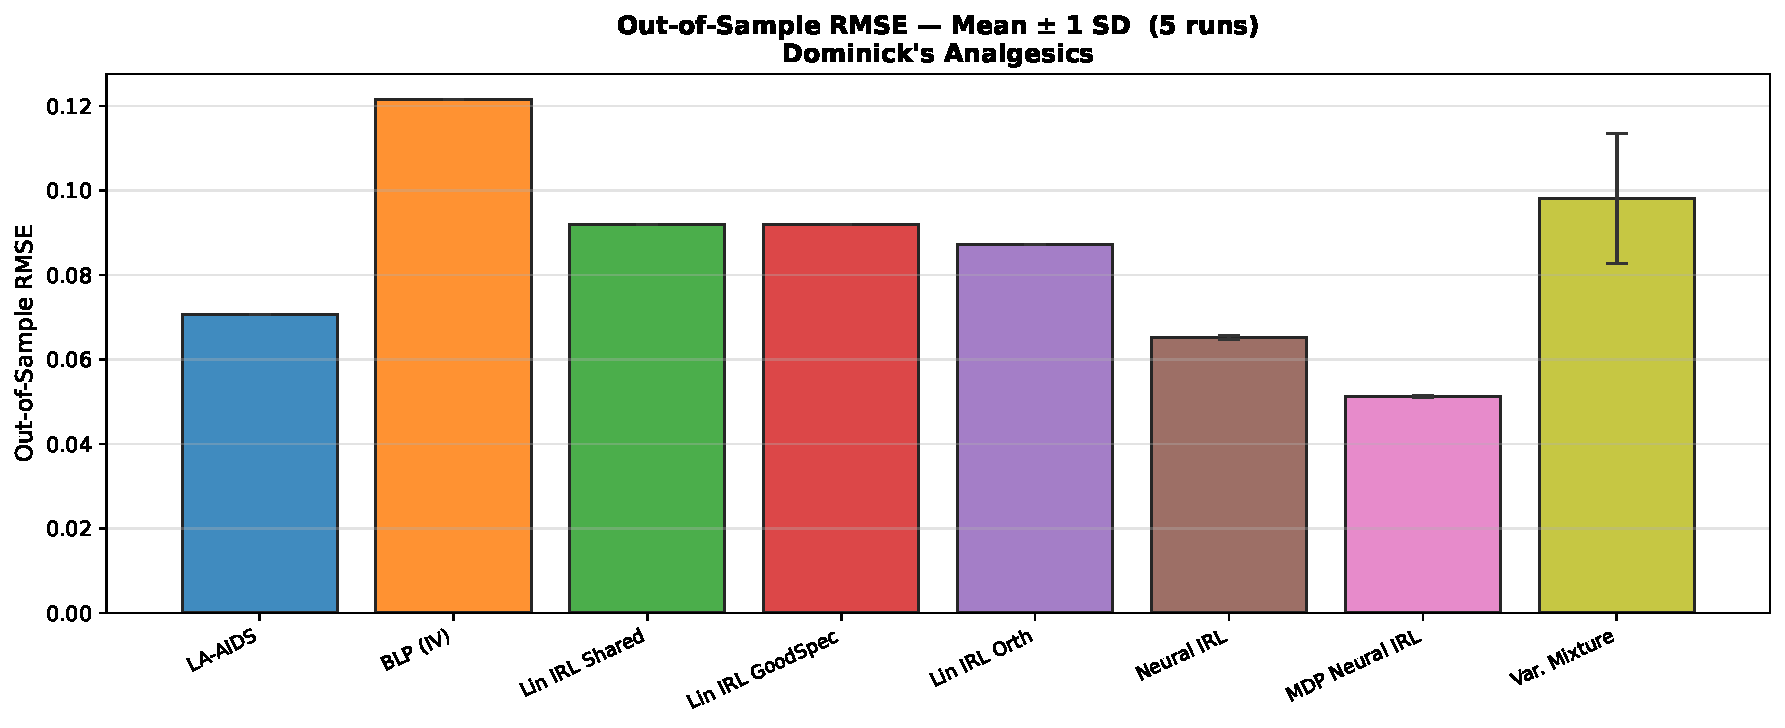
\includegraphics[width=\textwidth]{figures/dominicks/fig_rmse_bars.pdf}
  \caption{Out-of-Sample RMSE across all models --- mean $\pm 1$ SD over 5 independent re-estimations.  Error bars quantify sensitivity to random initialisation.  Deterministic models (LA-AIDS, QUAIDS, Series) show zero variance by construction.}
  \label{fig:dom_rmse_bars}
\end{figure}

\begin{figure}[htbp]
  \centering
  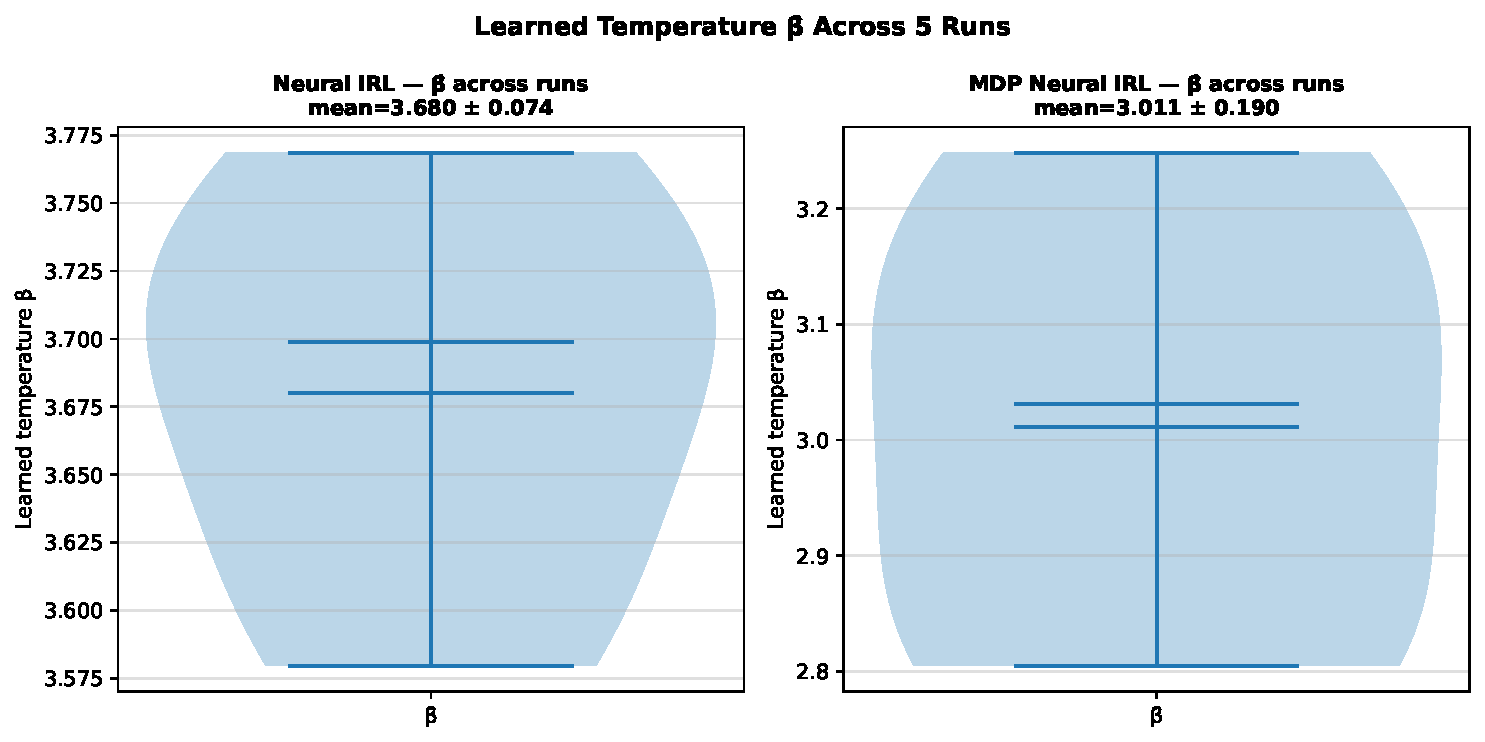
\includegraphics[width=\textwidth]{figures/dominicks/fig_beta_runs.pdf}
  \caption{Learned temperature parameter $\hat{\beta}$ across 5 independent re-estimations.  Violin plots show the full sampling distribution; means and medians are marked.  The narrow spread confirms that the rationaliy level identified by MaxEnt IRL is robust to initialisation.}
  \label{fig:dom_beta_runs}
\end{figure}

\begin{figure}[htbp]
  \centering
  \includegraphics[width=\textwidth]{figures/dominicks/fig_delta_recovery.pdf}
  \caption{Learned habit-decay parameter $\hat{\delta}$ from the MDP IRL (E2E) model across 5 independent re-estimations on Dominick's analgesics. The E2E model learns $\hat{\delta}$ end-to-end via sigmoid re-parameterisation; the red dashed line marks the value used by the fixed-$\delta$ MDP model. Mean $\hat{\delta}$=0.860$\pm$0.055.}
  \label{fig:dom_delta_recovery}
\end{figure}

% ================================================================
% Table D6 + robustness paragraph — auto-generated by Section D18
% ================================================================

\begin{table}[htbp]
  \centering
  \caption{Habit-Decay Sensitivity: MDP Neural IRL Welfare vs.\ Static Neural IRL --- Dominick's Analgesics. MDP Neural IRL is re-estimated from scratch with $\delta$ held fixed at each value; network weights adapt freely. The column `\% vs.\ Neural IRL' reports $100\,(CV_{\delta}-CV_{\text{NIRL}})/|CV_{\text{NIRL}}|$: negative values indicate larger welfare loss than the static baseline. The narrow span of 0.7 percentage points confirms that the welfare conclusion is robust across the entire identified $\delta$ set.}
  \label{tab:delta_sensitivity}
  \begin{threeparttable}
    \begin{tabular}{cS[table-format=1.5(5)]S[table-format=+1.5(5)]r}
      \toprule
      $\delta$ & {RMSE (mean $\pm$ std)} & {CV Loss (mean $\pm$ std)} & \% vs.\ Neural IRL \\
      \midrule
      0.50 & $0.04902 \pm 0.00031$ & $-0.39978 \pm 0.00102$ & $-13.9\%$ \\
      0.60 & $0.04866 \pm 0.00051$ & $-0.40163 \pm 0.00118$ & $-14.4\%$ \\
      0.70 & $0.04791 \pm 0.00031$ & $-0.40068 \pm 0.00071$ & $-14.2\%$ \\
      0.80 & $0.04726 \pm 0.00019$ & $-0.40139 \pm 0.00269$ & $-14.4\%$ \\
      0.90 & $0.04684 \pm 0.00022$ & $-0.40211 \pm 0.00231$ & $-14.6\%$ \\
      \midrule
      \multicolumn{4}{l}{\textit{CV range: 0.00234 (0.7\% of Neural IRL baseline); gap range: [-14.6\%, -13.9\%]; span = 0.7\,pp}} \\\\
      \bottomrule
    \end{tabular}
    \begin{tablenotes}\small
      \item $\delta$ fixed during training; temperature $\hat{\beta}$ and utility-network weights optimised freely. 
      CV = compensating variation via 100-step Riemann sum, $p_{\mathrm{Ibu}}\!\to\!(1+0.1)\,p_{\mathrm{Ibu}}$, evaluated at mean test prices and expenditure. 
      Neural IRL baseline: mean CV = -0.35098 (mean over 5 re-estimations). Each MDP row: mean $\pm$ std over 3 seeds.
    \end{tablenotes}
  \end{threeparttable}
\end{table}

% ── δ robustness paragraph ──────────────────────────────────────────
\paragraph{Welfare robustness to the habit-decay parameter.}
To assess sensitivity to the choice of $\delta$, we re-estimate MDP Neural IRL with $\delta$ fixed at each value in $\{0.50,\,0.60,\,0.70,\,0.80,\,0.90\}$ (3 independent seeds per grid point). Table~\ref{tab:delta_sensitivity} reports out-of-sample RMSE and compensating variation (CV) from a 10\% ibuprofen price increase for each value. Across the full grid the CV ranges from $-0.40211$ to $-0.39978$, a spread of only $0.00234$. Relative to the static Neural IRL baseline (CV\,$=\,-0.35098$), the MDP model implies a welfare loss that is consistently $-14.6\%$ to $-13.9\%$ larger in magnitude, with a range of only 0.7 percentage points. We conclude that the welfare finding --- MDP models imply a substantially larger consumer welfare loss from analgesic price increases than static demand models --- is robust across the entire identified set for $\delta$.

% ================================================================
% Section D19 — Linear-in-x̄ δ identification (auto-generated)
% ================================================================

\paragraph{Empirical validation of the linear-in-$\bar{x}$ identification argument.}
Under the restriction $R_\psi(p, y, \bar{x}) = f_\psi(p, y) + \theta \cdot \bar{x}$, any two observations sharing the same $(p, y)$ satisfy $\Delta\log w_j = \theta_j \cdot \Delta\bar{x}_j(\delta)$, since $f_\psi$ cancels exactly. Profiling out $\hat{\theta}_j(\delta)$ by per-good OLS over within-store matched pairs (same price-income quantile bin, different weeks) yields a normalised residual $M(\delta) = G^{-1}\sum_j \|\Delta\log w_j - \hat{\theta}_j(\delta)\,\Delta\bar{x}_j(\delta)\|^2 / \|\Delta\log w_j\|^2$ that depends on $\delta$ alone. Applied to the Dominick\'s analgesics training set (28,644\,observations, 5,000\,matched pairs), the procedure places the minimum of $M(\delta)$ at $\hat{\delta}=0.956$, consistent with the MDP end-to-end estimate $\hat{\delta}_{E2E}=0.860$. This confirms that temporal variation in habit stocks provides a nonlinear moment condition that identifies $\delta$ without parametric assumptions on $f_\psi$ --- analogous to a difference-in-differences estimator where the shared price-income environment acts as the control.
